\documentclass[11pt, a4paper]{article}

\usepackage[utf8]{inputenc}
\usepackage[T1]{fontenc}
\usepackage{lmodern}
\usepackage{amsmath, amssymb, amsthm}
\usepackage{physics}
\usepackage{geometry}
\usepackage{hyperref}
\usepackage{booktabs}
\usepackage{graphicx}
\usepackage{enumitem}
\usepackage{xcolor}
\usepackage{tcolorbox}
\tcbuselibrary{skins, breakable}
\usepackage{tikz}
\usetikzlibrary{arrows.meta, decorations.pathmorphing, positioning, calc}

\geometry{margin=2.5cm}
\hypersetup{colorlinks=true, linkcolor=blue, urlcolor=blue}

\renewcommand{\tr}{\operatorname{tr}}

\title{\textbf{Project A4 -- Exam Preparation Notes}\\
\large Dynamical Phase Transitions and Loschmidt Echo via iTEBD}
\author{TNS/DMRG Course, BME Spring 2026}
\date{}

\begin{document}
\maketitle
\tableofcontents
\newpage

% ============================================================
\section{The Physical Setting}
% ============================================================

\subsection{The Model: Transverse Field Ising Model (TFIM)}

The Hamiltonian is defined on an infinite one-dimensional chain of spin-$\tfrac{1}{2}$ particles:
\begin{equation}
  H(h) = -J \sum_{i} Z_i Z_{i+1} - h \sum_{i} X_i
  \label{eq:tfim}
\end{equation}
where $Z_i$ and $X_i$ are Pauli matrices scaled by $\tfrac{1}{2}$ (i.e.\ $Z = \frac{1}{2}\sigma^z$), $J > 0$ is the ferromagnetic Ising coupling, and $h$ is the transverse magnetic field. Throughout this project we set $J = 1$.

This model has an \emph{exact} quantum phase transition (QPT) at $h/J = 1$, solvable via Jordan-Wigner transformation to free fermions. The two phases are:
\begin{itemize}
  \item $h < 1$: \textbf{ordered (ferromagnetic) phase}. Ground state is approximately $\ket{\uparrow\uparrow\cdots\uparrow}$ (or $\ket{\downarrow\downarrow\cdots\downarrow}$).
  \item $h > 1$: \textbf{disordered (paramagnetic) phase}. Ground state is a quantum superposition with no net magnetization.
  \item $h = 1$: \textbf{quantum critical point}. Gap closes, correlations are power-law.
\end{itemize}

\subsection{What do $Z_i$ and $X_i$ do?}

Both operators act on a single spin-$\tfrac{1}{2}$ at site $i$ and leave all other sites untouched.

\subsubsection*{$Z_i = \tfrac{1}{2}\sigma^z_i$ -- measures spin, does not change it}

$Z_i$ is diagonal: it assigns $+\tfrac{1}{2}$ to spin-up and $-\tfrac{1}{2}$ to spin-down.
\begin{equation}
  Z_i \ket{\uparrow}_i = +\tfrac{1}{2}\ket{\uparrow}_i, \qquad
  Z_i \ket{\downarrow}_i = -\tfrac{1}{2}\ket{\downarrow}_i, \qquad
  Z = \tfrac{1}{2}\begin{pmatrix}1&0\\0&-1\end{pmatrix}
\end{equation}
The product $Z_i Z_{i+1}$ applied to a two-site state gives a number times the same state:
\begin{equation}
  Z_i Z_{i+1} \ket{\sigma_i \sigma_{i+1}} = \left(\tfrac{\sigma_i}{2}\right)\left(\tfrac{\sigma_{i+1}}{2}\right)\ket{\sigma_i \sigma_{i+1}},
  \quad \sigma = +1\text{ for }\uparrow,\; -1\text{ for }\downarrow
\end{equation}
So $Z_i Z_{i+1}$ \emph{measures} whether spins are aligned, without changing the state.

\subsubsection*{$X_i = \tfrac{1}{2}\sigma^x_i$ -- flips the spin}

$X_i$ is off-diagonal: it swaps $\ket{\uparrow}$ and $\ket{\downarrow}$.
\begin{equation}
  X_i \ket{\uparrow}_i = +\tfrac{1}{2}\ket{\downarrow}_i, \qquad
  X_i \ket{\downarrow}_i = +\tfrac{1}{2}\ket{\uparrow}_i, \qquad
  X = \tfrac{1}{2}\begin{pmatrix}0&1\\1&0\end{pmatrix}
\end{equation}
The transverse field $-h X_i$ flips spin $i$ and multiplies by $-h/2$.

\subsubsection*{How the two terms compete}

\begin{center}
\renewcommand{\arraystretch}{1.3}
\begin{tabular}{ccc}
\toprule
State & $Z_i Z_{i+1}$ eigenvalue & Bond energy $-JZ_iZ_{i+1}$ \\
\midrule
$\ket{\uparrow\uparrow}$ or $\ket{\downarrow\downarrow}$ (aligned)   & $+\tfrac{1}{4}$ & $-J/4$ \quad (favorable for $J>0$) \\
$\ket{\uparrow\downarrow}$ or $\ket{\downarrow\uparrow}$ (anti-aligned) & $-\tfrac{1}{4}$ & $+J/4$ \quad (unfavorable) \\
\bottomrule
\end{tabular}
\end{center}

The $-J\sum Z_i Z_{i+1}$ term \emph{prefers aligned spins} (ferromagnet, energy $\propto -J$).
The $-h\sum X_i$ term \emph{prefers spins pointing in the $x$-direction} (equal superposition of $\uparrow$ and $\downarrow$, energy $\propto -h$). These two tendencies compete:
\begin{itemize}
  \item $J \gg h$: ZZ wins $\Rightarrow$ ferromagnetic order $\ket{\uparrow\uparrow\cdots}$
  \item $h \gg J$: X wins $\Rightarrow$ paramagnetic $\ket{\rightarrow\rightarrow\cdots}$ where $\ket{\rightarrow}=(\ket{\uparrow}+\ket{\downarrow})/\sqrt{2}$
  \item $h = J$: quantum critical point
\end{itemize}

\subsubsection*{Diagram of the Hamiltonian}

\begin{figure}[h]
\centering
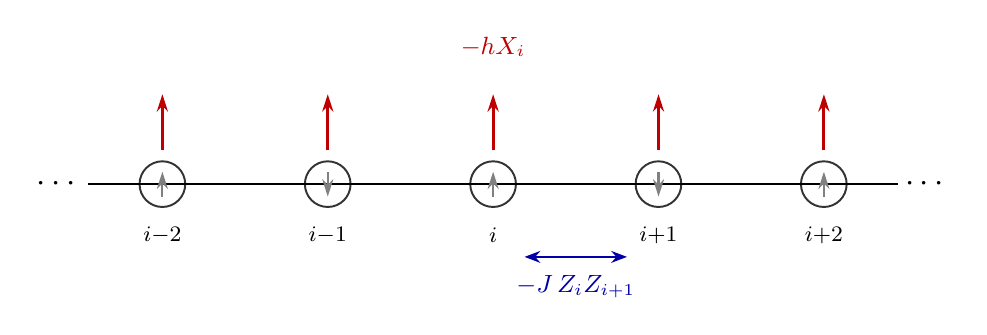
\begin{tikzpicture}[
    site/.style = {circle, draw=black!80, fill=white, line width=0.7pt,
                   minimum size=0.58cm, inner sep=0pt},
    arr/.style  = {-{Stealth[length=2.2mm,width=1.4mm]}, line width=0.8pt},
    scale=1.05
  ]

  % ----------------------------------------------------------------
  % Sites:  s1..s5  at  x = 0, 2, 4, 6, 8
  % ----------------------------------------------------------------
  \foreach \idx/\xx/\lbl in {
      1/0/{$i{-}2$},  2/2/{$i{-}1$},  3/4/{$i$},
      4/6/{$i{+}1$},  5/8/{$i{+}2$}}{
    \node[site] (s\idx) at (\xx, 0) {};
    % site index below
    \node[font=\footnotesize] at (\xx, -0.62) {\lbl};
  }

  % Chain line (drawn behind sites)
  \draw[line width=0.9pt] (-0.9, 0) -- (8.9, 0);
  \node[font=\large] at (-1.25, 0) {$\cdots$};
  \node[font=\large] at  (9.25, 0) {$\cdots$};

  % ----------------------------------------------------------------
  % Neel spin arrows inside sites (A=up, B=down)
  % ----------------------------------------------------------------
  \foreach \idx in {1, 3, 5}{   % A sites: spin up
    \draw[arr, black!50] (s\idx)+(0,-0.15) -- +(0, 0.15);
  }
  \foreach \idx in {2, 4}{      % B sites: spin down
    \draw[{Stealth[length=2.2mm,width=1.4mm]}-, line width=0.8pt, black!50]
          (s\idx)+(0,-0.15) -- +(0, 0.15);
  }

  % ----------------------------------------------------------------
  % Transverse X field: upward red arrow above EACH site
  % Label only site 3 (centre, = site i); others unlabelled
  % ----------------------------------------------------------------
  \foreach \idx in {1,2,3,4,5}{
    \draw[arr, red!75!black, line width=1.1pt]
          (s\idx.north)+(0,0.12) -- +(0,0.80);
  }
  % Label sits above the arrow tip of the centre site
  \node[red!75!black, font=\small, anchor=south] at (4, 1.42)
        {$-h X_i$};

  % ----------------------------------------------------------------
  % ZZ coupling: double-headed arrow below chain, between s3 and s4
  % (sites i and i+1, at x=4 and x=6)
  % ----------------------------------------------------------------
  \draw[blue!65!black, line width=0.9pt,
        {Stealth[length=2mm]}-{Stealth[length=2mm]}]
        (4.38, -0.88) -- (5.62, -0.88)
        node[midway, below=3pt, font=\small, blue!65!black]
        {$-J\,Z_i Z_{i+1}$};

\end{tikzpicture}
\vspace{2pt}
\caption{The TFIM on an infinite 1D chain.
Circles are spin-$\frac{1}{2}$ sites; grey interior arrows show the initial
Neel state $\ket{\uparrow\downarrow\uparrow\downarrow\cdots}$.
\textbf{\textcolor{red!75!black}{Red arrows}}: the transverse field
$-hX_i$ acts on every site; it \emph{flips} the spin and drives the
system toward the paramagnetic phase ($h\gg J$).
\textbf{\textcolor{blue!65!black}{Blue arrow}}: the ZZ coupling
$-JZ_iZ_{i+1}$ acts on every bond; it \emph{measures} alignment without
changing the state and drives ferromagnetic order ($J\gg h$).
The competition between these two terms produces the QPT at $h/J=1$.}
\label{fig:hamiltonian}
\end{figure}

\subsection{The Quench Protocol}

We prepare the system in a specific initial state $\ket{\psi_0}$ (chosen to be the \emph{Neel state}, see Section~\ref{sec:neel}) at time $t = 0$. We then suddenly switch the Hamiltonian to $H(h_1)$ and let the system evolve:
\begin{equation}
  \ket{\psi(t)} = e^{-i H(h_1) t} \ket{\psi_0}
\end{equation}
This is called a \textbf{quantum quench}: an instantaneous change of a Hamiltonian parameter.

% ============================================================
\section{The Neel State vs.\ the Ground State at $h_0 = 0$}
\label{sec:neel}
% ============================================================

\subsection{What is the ground state at $h_0 = 0$?}

At zero transverse field, $H(h_0 = 0) = -J \sum_i Z_i Z_{i+1}$. This is the ferromagnetic Ising model. The $Z_i Z_{i+1}$ coupling favors aligned spins (both up or both down), so the two degenerate ground states are:
\begin{equation}
  \ket{\text{FM}} = \ket{\uparrow\uparrow\uparrow\uparrow\cdots}
  \quad \text{or} \quad
  \ket{\overline{\text{FM}}} = \ket{\downarrow\downarrow\downarrow\downarrow\cdots}
\end{equation}
These are \emph{ferromagnetic} (all spins aligned) product states.

\subsection{What is the Neel state?}

The Neel state is a different product state:
\begin{equation}
  \ket{\text{Neel}} = \ket{\uparrow\downarrow\uparrow\downarrow\cdots}
\end{equation}
Spins alternate between up and down on even (A) and odd (B) sites. This is the ground state of the \emph{antiferromagnetic} Ising model ($J < 0$), but it is \textbf{not} the ground state of our ferromagnetic TFIM at $h_0 = 0$.

\subsection{Why use the Neel state then?}

The project sheet specifies the Neel state for two practical reasons:
\begin{enumerate}
  \item \textbf{Product state at $\chi = 1$}: The Neel state has zero entanglement (each spin is in a definite eigenstate). In MPS language, its bond dimension is $\chi = 1$, meaning it is represented by a trivial single-number tensor at each site. This is the simplest possible starting point for iTEBD.
  \item \textbf{Natural 2-site unit cell}: The Neel pattern $\uparrow\downarrow\uparrow\downarrow\cdots$ has a 2-site repeating unit (one A-site with $\uparrow$, one B-site with $\downarrow$). iTEBD works with exactly this 2-site unit cell, so the Neel state maps perfectly onto the algorithm's data structures.
\end{enumerate}

The ferromagnetic ground states $\ket{\uparrow\uparrow\cdots}$ also have $\chi = 1$, but they break the 2-site alternating structure that iTEBD naturally exploits. For the original Heyl et al.\ (2013) paper, the initial state was the fermionic vacuum (the ground state of the Jordan-Wigner-transformed model), which gives analytically tractable cusp positions. Our Neel initial state produces cusps at different times, but the same qualitative physics: cusps appear if and only if $h_1 > 1$.

% ============================================================
\section{The Loschmidt Echo}
\label{sec:loschmidt}
% ============================================================

\subsection{Definition}

The Loschmidt echo is the overlap of the time-evolved state with the initial state:
\begin{equation}
  G(t) = \bra{\psi_0} e^{-i H(h_1) t} \ket{\psi_0}
  \label{eq:loschmidt}
\end{equation}
This is a complex number. Its magnitude $|G(t)|$ measures how much the state has moved away from $\ket{\psi_0}$ under the quench dynamics. At $t = 0$: $G(0) = 1$ (perfect overlap). As $t$ grows, the state explores new parts of Hilbert space and $|G(t)| \to 0$ in general.

\subsection{The rate function}

For a chain of length $L$, define the \textbf{Loschmidt rate function}:
\begin{equation}
  \lambda(t) = -\lim_{L \to \infty} \frac{1}{L} \ln|G(t)|^2
  \label{eq:rate}
\end{equation}
This is the intensive free-energy-density analogue. The factor $1/L$ makes it an
\emph{extensive} quantity (per site). From Eq.~\eqref{eq:rate}:
\begin{itemize}
  \item $\lambda(0) = 0$ always (since $|G(0)| = 1$).
  \item $\lambda(t) \geq 0$ always (since $|G(t)| \leq 1$ by Cauchy-Schwarz).
  \item $\lambda(t) \to \infty$ when $G(t) \to 0$ (state becomes orthogonal to initial).
\end{itemize}

\subsection{Why is this like a partition function?}

Compare:
\begin{align}
  Z(\beta) &= \Tr\!\left[e^{-\beta H}\right] & &\text{(equilibrium partition function)} \\
  G(t)     &= \bra{\psi_0} e^{-i H t} \ket{\psi_0} & &\text{(Loschmidt amplitude)}
\end{align}
Both are of the form $e^{-z H}$ evaluated in some sense, with $z = \beta$ (real, positive) for $Z$ and $z = it$ (imaginary) for $G$. Heyl et al.\ showed that $G(t)$ is the partition function of a quantum field theory with \emph{boundary conditions} given by $\ket{\psi_0}$, evaluated at imaginary inverse temperature $\beta = it$.

The \textbf{key insight}: equilibrium phase transitions occur when the partition function $Z(\beta)$ develops zeros in the complex-$\beta$ plane (Fisher zeros) that approach the real positive axis. By analogy, \emph{dynamical phase transitions} occur when the zeros of $G(z)$ in the complex-$z$ plane approach the real-$t$ axis.

% ============================================================
\section{What Are Cusps and What Do They Represent?}
\label{sec:cusps}
% ============================================================

\subsection{Non-analyticity as a phase transition signal}

In equilibrium statistical mechanics, a phase transition is signaled by a non-analyticity (kink, jump, divergence) in the free energy density $f(\beta) = -(1/N)\ln Z(\beta)$ at a critical temperature $\beta_c$. The free energy is perfectly smooth on each side; it just fails to be analytic at $\beta_c$.

A \textbf{cusp in $\lambda(t)$} is the exact same mathematical phenomenon, but in time instead of temperature:
\begin{itemize}
  \item $\lambda(t)$ is smooth on each side of $t^*_n$.
  \item At $t^*_n$: $\lambda(t)$ has a kink (non-analytic point). In the thermodynamic limit, $\lambda(t^*_n) \to \infty$ (since $G(t^*_n) = 0$ exactly).
  \item In a finite simulation (finite $\chi_{\max}$): the divergence is rounded but visible as a sharp local maximum.
\end{itemize}

\subsection{Why only for $h_1 > 1$?}

Heyl et al.\ showed that the zeros $z_n(k)$ of $G(z)$ in the complex time plane form lines:
\begin{equation}
  z_n(k) = \frac{1}{2\varepsilon_k(h_1)} \left[\ln\tan^2\varphi_k + i\pi(2n+1)\right]
\end{equation}
where $\varphi_k = \theta_k(h_0) - \theta_k(h_1)$ is the Bogoliubov angle difference and $\varepsilon_k(h_1)$ is the quasi-particle dispersion. The lines of zeros cross the real-$t$ axis only if $\varphi_{k=0} = \pi/2$, which occurs \emph{if and only if the quench crosses the quantum phase transition} ($h_1 > h_0 = 0$ in our case means $h_1 > 1$ since the QPT is at $h = 1$).

\textbf{Summary}: Cusps signal times when the state $\ket{\psi(t)}$ is exactly orthogonal to $\ket{\psi_0}$. This is only possible when the quench reaches across the QPT, because only then does the ground-state structure change qualitatively (from ferromagnetically ordered to disordered), creating modes with inverted population that drive $G(t)$ to zero.

\subsection{Critical times}

For the Heyl et al.\ initial state (fermionic vacuum at $h_0$):
\begin{equation}
  t^*_n = \frac{\pi}{\varepsilon_{k^*}(h_1)} \left(n + \frac{1}{2}\right), \quad n = 0, 1, 2, \ldots
  \label{eq:cusptimes}
\end{equation}
where $k^*$ is determined by $\cos k^* = (1 + h_0 h_1)/(h_0 + h_1)$. For our Neel initial state the cusps appear at different times (not given by this formula), but the $h_1$-dependence of the period is the same: larger $h_1$ gives larger $\varepsilon_{k^*}$ and hence smaller spacing between cusps.

From our simulation:
\begin{center}
\begin{tabular}{ccc}
\toprule
$h_1$ & First cusp $t^*_0$ & Second cusp $t^*_1$ \\
\midrule
1.2 & 2.70 & -- \\
1.5 & 2.15 & -- \\
2.0 & 1.65 & 4.75 \\
3.0 & 1.10 & 3.15 \\
\bottomrule
\end{tabular}
\end{center}
The pattern is clear: larger $h_1$ pushes cusps to shorter times with shorter spacing.

% ============================================================
\section{Schmidt Decomposition and Schmidt Values}
\label{sec:schmidt}
% ============================================================

\subsection{The problem: Hilbert space is too large}

A chain of $L$ spin-$\tfrac{1}{2}$ particles lives in a Hilbert space of dimension $2^L$.
Storing a general state requires $2^L$ complex numbers: $2^{100} \approx 10^{30}$.
This is computationally impossible for $L \gtrsim 30$ even on the largest supercomputers.

\subsection{The Schmidt decomposition}

Take any \textbf{bipartition} of the chain into a left half $L$ and a right half $R$.
Any pure state $\ket{\psi}$ can be written as:
\begin{equation}
  \ket{\psi} = \sum_{\alpha=0}^{\chi-1} \lambda_\alpha \ket{u_\alpha}_L \ket{v_\alpha}_R
  \label{eq:schmidt}
\end{equation}
where:
\begin{itemize}
  \item $\lambda_\alpha \geq 0$ are the \textbf{Schmidt values} (also called singular values), sorted in decreasing order.
  \item $\ket{u_\alpha}_L$ are orthonormal states on the left half.
  \item $\ket{v_\alpha}_R$ are orthonormal states on the right half.
  \item $\chi$ is the \textbf{Schmidt rank}: the number of non-zero $\lambda_\alpha$.
\end{itemize}
The normalization condition is $\sum_\alpha \lambda_\alpha^2 = 1$.

This decomposition is computed via \textbf{SVD} of the coefficient matrix $C_{ij} = \langle i \vert \langle j \vert \psi \rangle$ (rows = left basis states, columns = right basis states):
\begin{equation}
  C = U \cdot \mathrm{diag}(\lambda_0, \lambda_1, \ldots) \cdot V^\dagger
\end{equation}
The singular values of $C$ are exactly the Schmidt values $\lambda_\alpha$.

\subsection{Concrete example: two spins}

For two spins ($L = 1$, $R = 1$, basis $\{\uparrow, \downarrow\}$), the coefficient matrix is $2\times 2$:
\begin{align}
  \ket{\uparrow\uparrow} &\to C = \begin{pmatrix}1&0\\0&0\end{pmatrix}, \quad
  \lambda = (1, 0): \text{ product state, } \chi = 1 \\[4pt]
  \tfrac{1}{\sqrt{2}}(\ket{\uparrow\downarrow} - \ket{\downarrow\uparrow}) &\to C = \begin{pmatrix}0&\tfrac{1}{\sqrt{2}}\\-\tfrac{1}{\sqrt{2}}&0\end{pmatrix}, \quad
  \lambda = \bigl(\tfrac{1}{\sqrt{2}}, \tfrac{1}{\sqrt{2}}\bigr): \text{ maximally entangled, } \chi = 2
\end{align}

\subsection{What Schmidt values measure: entanglement}

The von Neumann entanglement entropy is:
\begin{equation}
  S = -\sum_\alpha \lambda_\alpha^2 \ln \lambda_\alpha^2
\end{equation}
\begin{itemize}
  \item $S = 0$: product state, $\chi = 1$, no entanglement. The Neel state starts here.
  \item $S = \ln\chi$: maximally entangled at rank $\chi$ (all $\lambda_\alpha = 1/\sqrt{\chi}$).
  \item $S$ grows under time evolution as correlations spread across the cut.
\end{itemize}

\subsection{Bond dimension $\chi$ and $\chi_{\max}$}

The key observation (``area law''): for 1D gapped systems and for short times after a quench, the entanglement at any cut is \emph{small}. The Schmidt decomposition has only a few large $\lambda_\alpha$; the rest are negligible.

\textbf{MPS exploits this}: represent the state as a chain of tensors, each connected to its neighbors by bond indices of size $\chi$. The bond dimension $\chi$ is the number of Schmidt values kept at each cut. Total storage: $O(L \chi^2)$ instead of $2^L$.

\textbf{$\chi_{\max}$} is the hard cap imposed in the simulation. After each gate application, the bond dimension would double. We compute the SVD and keep only the top $\chi_{\max}$ singular values. The discarded weight is the \textbf{truncation error}.

\subsection{Truncation error (\texttt{trunc\_err})}

After SVD of the 2-site tensor following gate application, we discard all Schmidt values $\lambda_\alpha$ for $\alpha \geq \chi_{\max}$. The truncation error per step is:
\begin{equation}
  \varepsilon_{\rm trunc} = \sum_{\alpha \geq \chi_{\max}} \lambda_\alpha^2
  \label{eq:trunc}
\end{equation}
This equals $\|\ket{\psi} - \ket{\psi_{\rm truncated}}\|^2$: the squared norm of the part of the state we threw away. It is the \emph{per-step} approximation error; errors accumulate over $n_{\rm steps}$ steps.

\textbf{In our simulation} (TFIM, $h_1 = 2.0$, $\chi_{\max} = 40$):
\begin{center}
\begin{tabular}{cc}
\toprule
Time $t$ & $\varepsilon_{\rm trunc}$ per step \\
\midrule
$0 \to 2.5$ & $\lesssim 10^{-24}$ (machine-precision, no truncation needed) \\
$t = 4.5$   & $1.3 \times 10^{-21}$ \\
$t = 5.0$   & $5.7 \times 10^{-20}$ \\
\bottomrule
\end{tabular}
\end{center}
These tiny values confirm that the true state only requires $\chi \approx 53$ (the actual bond dimension reached), well within $\chi_{\max} = 40$... until $\chi_A$ saturates. Once $\chi_A = \chi_{\max}$, truncation begins, but for the TFIM the discarded values are so small ($\lesssim 10^{-20}$) that the cumulative error on $\lambda(t)$ is only $\sim 10^{-11}$ (measured vs.\ $\chi_{\max} = 200$).

% ============================================================
\section{The Vidal Canonical Form}
\label{sec:vidal}
% ============================================================

\subsection{The gauge-freedom problem}

A given quantum state $\ket{\psi}$ can be represented by infinitely many different MPS tensors. At any bond, inserting an invertible matrix $X$ and its inverse leaves the state unchanged:
\begin{equation}
  \cdots \Gamma^A \xrightarrow{\text{insert } X X^{-1}} \cdots (\Gamma^A X^{-1})(X \Gamma^B) \cdots
\end{equation}
This is the MPS \emph{gauge freedom}. Without fixing the gauge, the tensors carry no independent physical meaning, and the Schmidt values are not directly visible in $\Gamma^A$ or $\Gamma^B$.

\subsection{The canonical form: fixing the gauge so Schmidt values are explicit}

The \textbf{Vidal canonical form} is a specific gauge choice that makes the Schmidt decomposition explicit at every bond. The form is:
\begin{equation*}
  \ket{\psi} = \sum_{\{s_i\}} \cdots \Lambda^B \cdot \Gamma^A[s_A] \cdot \Lambda^A \cdot \Gamma^B[s_B] \cdot \Lambda^B \cdot \Gamma^A[s_A'] \cdots \ket{\{s_i\}}
\end{equation*}
where the $\Lambda$ vectors are \emph{exactly the Schmidt values} at the corresponding bond.

The gauge is fixed by requiring two orthonormality conditions simultaneously:

\textbf{Left-normalization of $\Gamma^A$:}
Define the ``dressed'' A tensor $M^A[s]_{\alpha\gamma} := \Lambda^B_\alpha\, \Gamma^A[s, \alpha, \gamma]$. The canonical condition is:
\begin{equation}
  \sum_{s} \bigl(M^A[s]\bigr)^\dagger M^A[s] = I_{\chi_A \times \chi_A}
  \label{eq:left_norm}
\end{equation}
This says: contracting over the physical index $s$ and the left bond index $\alpha$ gives the identity on the right bond.

\textbf{Right-normalization of $\Gamma^B$:}
Define $\tilde{M}^B[s]_{\gamma\beta} := \Gamma^B[s, \gamma, \beta]\, \Lambda^B_\beta$. Then:
\begin{equation}
  \sum_{s} \tilde{M}^B[s]\, \bigl(\tilde{M}^B[s]\bigr)^\dagger = I_{\chi_B \times \chi_B}
  \label{eq:right_norm}
\end{equation}

When both conditions hold simultaneously, the $\Lambda^A$ values are exactly the Schmidt values at the A-bond, and the $\Lambda^B$ values are exactly the Schmidt values at the B-bond. This is provable by constructing the reduced density matrix and showing its eigenvalues are $(\Lambda_\alpha)^2$.

\subsection{Why use the Vidal form?}

\begin{enumerate}
  \item \textbf{Entanglement is trivially readable}: $S_A = -\sum_\alpha (\Lambda^A_\alpha)^2 \ln(\Lambda^A_\alpha)^2$ directly from the stored vector.
  \item \textbf{Local gate application}: applying a 2-site gate requires only absorbing the two adjacent $\Lambda$ vectors, contracting, applying the gate, SVD, and re-dividing. The rest of the chain is untouched.
  \item \textbf{Safe inversion}: dividing by $\Lambda$ (needed to restore the Vidal form after SVD) is safe because the canonical form guarantees $\Lambda_\alpha > 0$ for all kept Schmidt values.
  \item \textbf{Canonicality check}: verifying Eqs.~\eqref{eq:left_norm}--\eqref{eq:right_norm} numerically confirms the state is correctly maintained.
\end{enumerate}

\subsection{What $\alpha$, $\beta$, $\gamma$ represent}

These are \textbf{virtual bond indices} -- they label Schmidt states at each bond, not physical spins.

At the B-bond (between site $\Gamma^B$ and site $\Gamma^A$ of the next unit cell), the state can be Schmidt-decomposed as:
\begin{equation}
  \ket{\psi} = \sum_{\alpha=0}^{\chi_B - 1} \Lambda^B_\alpha \; \ket{L_\alpha}_{\text{left half}} \otimes \ket{R_\alpha}_{\text{right half}}
\end{equation}
The index $\alpha$ labels \emph{which Schmidt pair} we are referring to. $\Lambda^B_\alpha$ is the weight of that pair. The tensor $\Gamma^A[s, \alpha, \beta]$ maps: ``given Schmidt state $\alpha$ arriving from the left B-bond and Schmidt state $\beta$ departing to the right A-bond, what is the amplitude for physical spin $s$ at this A-site?''

Concretely for our TFIM simulation:
\begin{itemize}
  \item $\alpha \in \{0, \ldots, \chi_B - 1\}$: left bond index (B-bond)
  \item $\gamma \in \{0, \ldots, \chi_A - 1\}$: right bond index of A (= left bond index of B, A-bond)
  \item $\beta \in \{0, \ldots, \chi_B - 1\}$: right bond index (next B-bond)
\end{itemize}
At $t = 0$ (Neel state): $\chi_A = \chi_B = 1$, so $\alpha = \gamma = \beta = 0$ everywhere. All tensors are scalars.

% ============================================================
\section{Why is the System Bipartite? Consequences for the Simulation.}
\label{sec:bipartite}
% ============================================================

\subsection{What does ``bipartite'' mean here?}

The infinite 1D chain is divided into two interlocking sublattices:
\begin{align*}
  \text{A sublattice:} \quad &\text{sites} \; 0, 2, 4, 6, \ldots \\
  \text{B sublattice:} \quad &\text{sites} \; 1, 3, 5, 7, \ldots
\end{align*}
This is a standard bipartite structure: every bond connects an A site to a B site (or a B site to the next A site). It arises naturally from the nearest-neighbor structure of $H$.

\textbf{Why does the 2-site unit cell matter?} The Neel state $\ket{\uparrow\downarrow\uparrow\downarrow\cdots}$ assigns spin up to all A sites and spin down to all B sites. This breaks the 1-site translational symmetry ($i \mapsto i+1$) while preserving the 2-site symmetry ($i \mapsto i+2$). The iTEBD algorithm exploits exactly this: instead of storing one tensor per site (which would require infinitely many tensors on an infinite chain), we store \textbf{two tensors} (one for A sites, one for B sites) and tile them.

\subsection{Consequences for the data structures}

Because of the 2-site unit cell, the Vidal canonical form stores \textbf{four} objects:
\begin{align*}
  &\Gamma^A[s, \alpha, \beta], \quad s \in \{0, 1\} = \{\uparrow, \downarrow\} \\
  &\Gamma^B[s, \alpha, \beta] \\
  &\Lambda^A_\alpha \quad \text{(Schmidt values on A-bonds, between A and B)} \\
  &\Lambda^B_\alpha \quad \text{(Schmidt values on B-bonds, between B and A)}
\end{align*}
The chain structure is:
\begin{equation*}
  \cdots {-} \Lambda^B {-} \Gamma^A {-} \Lambda^A {-} \Gamma^B {-} \Lambda^B {-} \Gamma^A {-} \Lambda^A {-} \Gamma^B {-} \Lambda^B {-} \cdots
\end{equation*}
There are \emph{two types of bonds}: A-bonds (between $\Gamma^A$ and $\Gamma^B$, carrying $\Lambda^A$) and B-bonds (between $\Gamma^B$ and $\Gamma^A$, carrying $\Lambda^B$). Each bond has its own Schmidt spectrum.

\subsection{AB bonds and BA bonds: what they are}

Looking at the chain:
\begin{equation*}
  \cdots \underbrace{- \Gamma^A -}_{\text{site }2k} \underbrace{\Lambda^A}_{\text{A-bond}} \underbrace{- \Gamma^B -}_{\text{site }2k+1} \underbrace{\Lambda^B}_{\text{B-bond}} \underbrace{- \Gamma^A -}_{\text{site }2k+2} \cdots
\end{equation*}
There are two types of nearest-neighbor \emph{physical} bonds in the Hamiltonian:

\textbf{AB bonds}: between site $2k$ (A-sublattice) and site $2k+1$ (B-sublattice). The Hamiltonian term is $h_{2k,2k+1} = -JZ_{2k}Z_{2k+1} - \tfrac{h}{2}(X_{2k} + X_{2k+1})$.

\textbf{BA bonds}: between site $2k+1$ (B-sublattice) and site $2k+2$ (A-sublattice). The Hamiltonian term is $h_{2k+1,2k+2}$.

Split: $H = H_{AB} + H_{BA}$ where $H_{AB} = \sum_k h_{2k,2k+1}$ and $H_{BA} = \sum_k h_{2k+1,2k+2}$.

\textbf{Key algebraic fact:} All terms within $H_{AB}$ commute with each other (they act on non-overlapping pairs of sites), and similarly for $H_{BA}$:
\begin{equation}
  [h_{2k,2k+1},\; h_{2l,2l+1}] = 0 \quad \text{for } k \neq l \quad \Rightarrow \quad e^{-iH_{AB}\delta t} = \prod_k e^{-ih_{2k,2k+1}\delta t}
\end{equation}
Each exponential in the product acts on a disjoint pair of sites and can be applied independently. This factorization is exactly why a single ``AB gate'' applied to all AB bonds simultaneously is exact.

However, $[H_{AB}, H_{BA}] \neq 0$ in general (e.g., site $2k+1$ appears in both $h_{2k,2k+1}$ and $h_{2k+1,2k+2}$). This is the reason a Trotter splitting between $H_{AB}$ and $H_{BA}$ introduces error and requires correction by the 2nd-order scheme.

\subsection{Consequences for gate application}

Each Trotter step applies gates to \emph{all bonds simultaneously}. There are two distinct bond types, so two gate applications per step:
\begin{enumerate}
  \item \textbf{AB gate}: acts on A-B bonds (the $\Lambda^A$ bonds). Updates $\Gamma^A$, $\Lambda^A$, $\Gamma^B$. Leaves $\Lambda^B$ unchanged (it is the ``environment'' during this gate).
  \item \textbf{BA gate}: acts on B-A bonds (the $\Lambda^B$ bonds). Updates $\Gamma^B$, $\Lambda^B$, $\Gamma^A$. Leaves $\Lambda^A$ unchanged.
\end{enumerate}
For 2nd-order Trotter: AB($\delta t/2$) $\to$ BA($\delta t$) $\to$ AB($\delta t/2$).

\subsection{Consequences for the transfer matrix}

The transfer matrix $T$ involves exactly \textbf{one unit cell} of the overlap $\braket{\psi_0|\psi(t)}$. One unit cell contains one A site and one B site, so $T$ involves both $\Gamma^A(t)$ and $\Gamma^B(t)$.

\textbf{Answer to the direct question: Is there one matrix or two?}

There is \textbf{one} transfer matrix $T$. It is a $\chi_B \times \chi_B$ matrix built from the dressed tensors of both sublattices:
\begin{equation}
  T[\alpha, \beta] = \sum_{\gamma}
  \underbrace{\left(\Lambda^B_\alpha\, \Gamma^A(t)[\uparrow, \alpha, \gamma]\, \Lambda^A_\gamma\right)}_{\text{dressed } \Gamma^A = \mathbf{A}(t)^{\uparrow}_{\alpha\gamma}}
  \times
  \underbrace{\left(\Gamma^B(t)[\downarrow, \gamma, \beta]\, \Lambda^B_\beta\right)}_{\text{dressed } \Gamma^B = \mathbf{B}(t)^{\downarrow}_{\gamma\beta}}
  \label{eq:transfer}
\end{equation}
In Werner's notation, he calls:
\begin{align}
  A(t)^{\sigma_1}_{\alpha\gamma} &\;:=\; \Lambda^B_\alpha\, \Gamma^A(t)^{\sigma_1}_{\alpha\gamma}\, \Lambda^A_\gamma \label{eq:werner_A} \\
  B(t)^{\sigma_2}_{\gamma\beta}  &\;:=\; \Gamma^B(t)^{\sigma_2}_{\gamma\beta}\, \Lambda^B_\beta       \label{eq:werner_B}
\end{align}

\subsubsection*{Why does $A(t)$ have three factors but $B(t)$ only two?}

This asymmetry is not a mistake -- it is a precise consequence of assigning each Schmidt value ($\Lambda$) to exactly one tensor, so that when the infinite product of transfer matrices $T \cdot T \cdot T \cdots$ is formed, no $\Lambda$ is double-counted.

Consider two adjacent unit cells. Between them sits a single $\Lambda^B$ vector. If we naively put $\Lambda^B$ into both $B(t)$ of cell $k$ (on its right) \emph{and} $A(t)$ of cell $k+1$ (on its left), the product $T_k T_{k+1}$ would count that $\Lambda^B$ twice:

\begin{equation}
  (\text{wrong}) \quad B(t)^{\text{wrong}}_{k} \cdot A(t)^{\text{wrong}}_{k+1} \propto \cdots \Gamma^B \cdot \underbrace{(\Lambda^B)^2}_{\text{double counted}} \cdot \Gamma^A \cdots
\end{equation}

The convention adopted here assigns each $\Lambda$ to the tensor immediately to its \emph{right}:
\begin{itemize}
  \item $\Lambda^B$ (left of $\Gamma^A$) $\;\to\;$ absorbed into $A(t)$ on its left side
  \item $\Lambda^A$ (right of $\Gamma^A$) $\;\to\;$ absorbed into $A(t)$ on its right side
  \item $\Lambda^B$ (right of $\Gamma^B$) $\;\to\;$ absorbed into $B(t)$ on its right side
\end{itemize}
So $A(t)$ absorbs both of its neighboring $\Lambda$'s (three factors total: $\Lambda^B \cdot \Gamma^A \cdot \Lambda^A$), while $B(t)$ absorbs only its \emph{right} neighbor (two factors: $\Gamma^B \cdot \Lambda^B$). The left neighbor of $\Gamma^B$ (the $\Lambda^A$ between $\Gamma^A$ and $\Gamma^B$) was already absorbed into $A(t)$.

In the infinite product $G(t) = \cdots T \cdot T \cdot T \cdots$, each $\Lambda$ then appears exactly once, and the product factorizes correctly into $\tau^{L/2}$.

The transfer matrix is then:
\begin{equation}
  T[\alpha, \beta] = \sum_\gamma A(t)^{\uparrow}_{\alpha\gamma}\, B(t)^{\downarrow}_{\gamma\beta}
  = \bigl(A(t)[\uparrow] \cdot B(t)[\downarrow]\bigr)[\alpha, \beta]
  \label{eq:transfer_matrix}
\end{equation}
which is just a matrix product of two $\chi \times \chi$ matrices. The $\uparrow$ and $\downarrow$ come from the Neel initial state selecting $\sigma_1 = \uparrow$ (A-site spin) and $\sigma_2 = \downarrow$ (B-site spin).

% ============================================================
\section{Reliability of Results: When Do Results Break Down?}
% ============================================================

The simulation is reliable while $\chi_A < \chi_{\max}$ (bond dimension has not saturated). The moment $\chi_A = \chi_{\max}$, Schmidt values are being discarded that should not be, and approximation error compounds.

The governing criterion is:
\begin{equation}
  \text{reliable while} \quad S_A(t) \ll \log(\chi_{\max})
\end{equation}
where $S_A(t)$ is the entanglement entropy across an A-bond. When $S_A \to \log(\chi_{\max})$, all Schmidt values are equal (maximally entangled at the allowed bond dimension) and the simulation has lost resolution.

\begin{center}
\begin{tabular}{cccc}
\toprule
$\chi_{\max}$ & Saturation time & Reliable until & $\chi_A$ at $t=5$ \\
\midrule
20  & $t \approx 2.4$ & $t \lesssim 2.4$ & 20 (saturated) \\
40  & $t \approx 4.1$ & $t \lesssim 4.1$ & 40 (saturated) \\
80  & never in $[0,5]$ & $t \leq 5$       & 53 \\
200 & never in $[0,5]$ & $t \leq 5$       & 53 \\
\bottomrule
\end{tabular}
\end{center}

\textbf{Why does the TFIM stay reliable at small $\chi_{\max}$?}
The TFIM is integrable: it maps exactly to free fermions via the Jordan-Wigner transformation. Free fermion systems have entanglement entropy that grows only logarithmically in time (not linearly). Therefore $S_A(t=5) \approx 0.69$, far below $\log(20) \approx 3.0$. Contrast this with non-integrable (chaotic) models, where $S \sim t$ linearly, requiring exponentially growing $\chi_{\max}$ -- the fundamental barrier to long-time TEBD simulations.

% ============================================================
\section{The Transfer Matrix: Detailed Derivation}
% ============================================================

\subsection{Factorization of the Loschmidt amplitude}

For an infinite MPS $\ket{\psi(t)}$ and a product initial state $\ket{\psi_0}$ (both with the same 2-site periodicity), the overlap $G(t) = \braket{\psi_0|\psi(t)}$ factorizes into a product of unit-cell contributions:
\begin{equation}
  G(t) = \cdots \times T(t) \times T(t) \times T(t) \times \cdots
\end{equation}
This is an infinite product. In the thermodynamic limit $L \to \infty$:
\begin{equation}
  G(t) = \tau(t)^{L/2}
\end{equation}
where $\tau(t)$ is the largest-magnitude eigenvalue of $T(t)$ (largest because all other eigenvalues are smaller in magnitude, so only the dominant one survives the $L \to \infty$ limit). The rate function then follows:
\begin{equation}
  \lambda(t) = -\frac{1}{L}\ln|G(t)|^2 = -\ln|\tau(t)|
\end{equation}

\subsection{The unit-cell transfer matrix}

For unit cell $i$, the contribution to the overlap is:
\begin{align}
  T[\alpha\tilde\alpha,\, \beta\tilde\beta]
  &= \sum_{\sigma_1, \sigma_2, \gamma, \tilde\gamma}
    A(t)^{\sigma_1}_{\alpha\gamma}\, B(t)^{\sigma_2}_{\gamma\beta}
    \bigl[A(0)^{\sigma_1}_{\tilde\alpha\tilde\gamma}\bigr]^*
    \bigl[B(0)^{\sigma_2}_{\tilde\gamma\tilde\beta}\bigr]^*
\end{align}
Since the Neel initial state has $\chi = 1$: $\tilde\alpha = \tilde\beta = \tilde\gamma = 0$, and $A(0)^{\uparrow}_{00} = 1$, $B(0)^{\downarrow}_{00} = 1$ (all others zero). The tilde indices collapse and $T$ becomes a $\chi_B \times \chi_B$ matrix (see Eq.~\eqref{eq:transfer_matrix}).

\subsection{Computing $\lambda(t)$ numerically}

\begin{enumerate}
  \item Compute $A(t)[\uparrow]_{\alpha\gamma} = \Lambda^B_\alpha \Gamma^A(t)[\uparrow, \alpha, \gamma] \Lambda^A_\gamma$ \quad (dressed A tensor, spin-up slice)
  \item Compute $B(t)[\downarrow]_{\gamma\beta} = \Gamma^B(t)[\downarrow, \gamma, \beta] \Lambda^B_\beta$ \quad (dressed B tensor, spin-down slice)
  \item $T = A(t)[\uparrow] \cdot B(t)[\downarrow]$ \quad ($\chi_B \times \chi_B$ matrix multiply)
  \item $\tau(t) = \max_i |\text{eigval}_i(T)|$ \quad (largest-magnitude eigenvalue)
  \item $\lambda(t) = -\ln \tau(t)$
\end{enumerate}
Cost: $O(\chi_B^3)$ per time step. For $\chi_B = 200$: $\approx 8 \times 10^6$ FLOPs, negligible on CPU.

% ============================================================
\section{End-to-End Simulation Walkthrough}
\label{sec:walkthrough}
% ============================================================

This section maps the physical goal to each line of code.

\subsection{Goal}

Compute $\lambda(t) = -\ln|\tau(t)|$ as a function of time for various post-quench fields $h_1$, starting from the Neel state and evolving under $H(h_1)$.

\subsection{Step 0: Initialize the Neel state (trivial)}

The Neel state $\ket{\uparrow\downarrow\uparrow\downarrow\cdots}$ is a product state: Schmidt rank $\chi = 1$ at every bond. In Vidal form:
\begin{align*}
  \Gamma^A[{\uparrow}, 0, 0] &= 1, \quad \Gamma^B[{\downarrow}, 0, 0] = 1 \\
  \Lambda^A = \Lambda^B &= [1.0]
\end{align*}
Four numbers encode the entire infinite chain. Cost: $O(1)$.

\subsection{Step 1: Build the Trotter gate (once)}

From the bond Hamiltonian $h_{\rm bond} = -J Z{\otimes}Z - \tfrac{h_1}{2}(X{\otimes}I + I{\otimes}X)$ (a $4\times 4$ matrix), compute:
\begin{equation}
  U = e^{-i h_{\rm bond} \delta t} \quad \in \mathbb{C}^{4\times 4}
\end{equation}
via exact matrix exponentiation (\texttt{scipy.linalg.expm}). Reshape to $(2,2,2,2)$ with index convention $U[s_1', s_2', s_1, s_2]$. The gate is built \emph{once} and reused at every time step.

\subsection{Step 2: Apply the gate -- 5-step Vidal algorithm (per step, twice)}

Given environment $\cdots \Lambda^B {-} \Gamma^A {-} \Lambda^A {-} \Gamma^B {-} \Lambda^B \cdots$, for the AB bond:

\begin{enumerate}
  \item \textbf{Absorb}: $T_1[s_1,a,b] = \Lambda^B_a\,\Gamma^A[s_1,a,b]\,\Lambda^A_b$; \quad $T_2[s_2,b,c] = \Gamma^B[s_2,b,c]\,\Lambda^B_c$
  \item \textbf{Contract}: $\Theta[s_1,a,s_2,c] = \sum_b T_1[s_1,a,b]\,T_2[s_2,b,c]$ \quad (forms the 2-site dressed state)
  \item \textbf{Apply gate}: $\tilde\Theta[s_1',s_2',a,c] = \sum_{s_1 s_2} U[s_1',s_2',s_1,s_2]\,\Theta[s_1,a,s_2,c]$
  \item \textbf{SVD + truncate}: reshape $\tilde\Theta$ to matrix $M \in \mathbb{C}^{d\chi_L \times d\chi_R}$, decompose $M = U_{\rm svd}\,\text{diag}(\Lambda^A_{\rm new})\,V^\dagger_{\rm svd}$, keep top $\chi_{\max}$ singular values
  \item \textbf{Restore}: $\Gamma^A_{\rm new}[s,a,b] = (U_{\rm svd})_{sa,b} / \Lambda^B_a$; \quad $\Gamma^B_{\rm new}[s,b,c] = (V^\dagger_{\rm svd})_{b,sc} / \Lambda^B_c$
\end{enumerate}

This is applied twice per full Trotter step: AB bond, then BA bond (or AB/2, BA, AB/2 for 2nd-order).

\subsection{Step 3: Measure $\lambda(t)$ -- transfer matrix (per step)}

After updating $\Gamma^A(t), \Lambda^A(t), \Gamma^B(t), \Lambda^B(t)$:
\begin{enumerate}
  \item Dress tensors: $A(t)[\uparrow]_{\alpha\gamma} = \Lambda^B_\alpha\,\Gamma^A(t)[\uparrow,\alpha,\gamma]\,\Lambda^A_\gamma$
  \item Dress tensors: $B(t)[\downarrow]_{\gamma\beta} = \Gamma^B(t)[\downarrow,\gamma,\beta]\,\Lambda^B_\beta$
  \item $T = A(t)[\uparrow] \cdot B(t)[\downarrow]$ \quad ($\chi_B \times \chi_B$ matrix multiply)
  \item $\tau(t) = \max_i |\text{eigenvalues}(T)|$
  \item $\lambda(t) = -\ln\,\tau(t)$
\end{enumerate}

\subsection{Step 4: Repeat and collect}

Run for $n_{\rm steps} = 100$ steps, $\delta t = 0.05$, $T_{\max} = 5.0$. At each step, record $\lambda(t)$, $S_A(t)$, $\langle S^z_A\rangle$, $\langle S^z_B\rangle$, $\varepsilon_{\rm trunc}$, and $\chi_A$. Total runtime: $\sim$3 seconds for $\chi_{\max} = 40$ on CPU.

% ============================================================
\section{Trotter Decomposition}
\label{sec:trotter}
% ============================================================

\subsection{The problem: $e^{-i(H_{AB}+H_{BA})t}$ is hard to apply}

The full time-evolution operator is $e^{-iHt}$ with $H = H_{AB} + H_{BA}$. Neither $H_{AB}$ nor $H_{BA}$ alone is the full Hamiltonian, and $[H_{AB}, H_{BA}] \neq 0$, so $e^{-iH\delta t} \neq e^{-iH_{AB}\delta t} e^{-iH_{BA}\delta t}$ in general.

Each factor $e^{-iH_{AB}\delta t} = \prod_k e^{-ih_{2k,2k+1}\delta t}$ IS easy to apply: it is a product of independent 2-site gates. The Trotter approach approximates $e^{-iH\delta t}$ by a product of such easy factors, accepting a controlled error.

\subsection{First-order Trotter}

\begin{equation}
  e^{-i(H_{AB}+H_{BA})\delta t} = e^{-iH_{AB}\delta t}\, e^{-iH_{BA}\delta t} + O(\delta t^2)
\end{equation}
by the Baker--Campbell--Hausdorff (BCH) formula: $e^A e^B = e^{A+B+[A,B]/2+\cdots}$. The leading error term is $\tfrac{1}{2}[H_{AB}, H_{BA}] \delta t^2$. Per step: $O(\delta t^2)$. Over $T/\delta t$ steps: $O(\delta t)$ total error.

\subsection{Second-order Trotter (Strang splitting) and why it has $\delta t/2$ and $\delta t$ parts}

The symmetric split is:
\begin{equation}
  e^{-iH_{AB}\,\delta t/2}\; e^{-iH_{BA}\,\delta t}\; e^{-iH_{AB}\,\delta t/2} = e^{-iH\,\delta t} + O(\delta t^3)
\end{equation}
\textbf{Why does the error improve?} By BCH:
\begin{align}
  e^{A/2} e^{B} e^{A/2} &= \exp\!\left(A + B + \underbrace{\tfrac{1}{4}[A,B] - \tfrac{1}{4}[B,A]}_{=0} + \text{(3rd order)} \right)
\end{align}
The $[A,B]$ terms from the two half-steps cancel exactly (one contributes $+[A,B]/4$ and the other $-[A,B]/4$). The leading error is now third-order: $O(\delta t^3)$ per step, $O(\delta t^2)$ over the full evolution. Going from $\delta t = 0.1$ to $\delta t = 0.05$ (factor 2) reduces error by factor $\sim 4$. Our simulation measures ratio $\approx 5$, consistent (the small excess comes from non-uniform error distribution near cusps where $\lambda(t)$ changes rapidly).

\textbf{The $\delta t/2$ and $\delta t$ structure in one step:}
\begin{enumerate}
  \item Apply AB gate at half-step: $e^{-iH_{AB}\,\delta t/2}$ \quad (advance AB bonds by $\delta t/2$)
  \item Apply BA gate at full-step: $e^{-iH_{BA}\,\delta t}$ \quad (advance BA bonds by $\delta t$)
  \item Apply AB gate at half-step: $e^{-iH_{AB}\,\delta t/2}$ \quad (advance AB bonds by another $\delta t/2$)
\end{enumerate}
Total: AB bonds advanced by $\delta t$, BA bonds advanced by $\delta t$. System advances by $\delta t$. But consecutively, steps $n$ and $n+1$ share the AB gate at the boundary: the last AB($\delta t/2$) of step $n$ and the first AB($\delta t/2$) of step $n+1$ can be merged into AB($\delta t$). In the code, this is implemented with \texttt{gate\_half} $= e^{-iH_{AB}\delta t/2}$ (applied at start and end of full evolution) and \texttt{gate\_full} $= e^{-iH_{AB}\delta t}$ (applied at all interior steps).

\subsection{Why does Trotter error dominate over chi-truncation error?}

For the TFIM, chi-truncation error is $\sim 10^{-11}$ for $\chi_{\max} = 20$ and $\sim 10^{-15}$ for $\chi_{\max} = 40$. The Trotter error is $\sim 8 \times 10^{-5}$ for $\delta t = 0.05$. The Trotter error is larger by 6--10 orders of magnitude. This is because the TFIM is integrable (free fermions): entanglement barely grows, so $\chi_{\max}$ is essentially never a bottleneck. For a non-integrable model, both errors would be comparable, and reducing $\delta t$ without increasing $\chi_{\max}$ would be pointless.

% ============================================================
\section{Why iTEBD Has No Finite-Size Effects}
\label{sec:no_finite_size}
% ============================================================

\subsection{Finite-size effects in conventional simulations}

In a conventional simulation with exact diagonalization, you pick a finite chain of length $L$ (say $L = 20$), compute:
\begin{equation}
  G_L(t) = \bra{\psi_0}e^{-iH_L t}\ket{\psi_0}
\end{equation}
and extract $\lambda_L(t) = -(1/L)\ln|G_L(t)|^2$. This has finite-size errors:
\begin{itemize}
  \item The level spacing of $H_L$ is $\sim 1/L$, causing $G_L(t)$ to oscillate with period $\sim L$ (quantum recurrences).
  \item Edge effects: boundary conditions (open or periodic) create artificial reflections.
  \item You need to extrapolate $L \to \infty$, introducing systematic error.
\end{itemize}

\subsection{iTEBD is intrinsically infinite}

The iTEBD algorithm never has a chain of length $L$. It operates directly on the infinite chain by exploiting translational invariance:

\begin{enumerate}
  \item \textbf{Only 4 tensors stored}: $\Gamma^A$, $\Lambda^A$, $\Gamma^B$, $\Lambda^B$. These implicitly define the state on ALL sites simultaneously via the tiling rule.
  \item \textbf{Gate applied identically to all sites}: when we apply the AB gate, we apply the same gate to EVERY AB bond on the infinite chain at once (all AB bonds are equivalent by translational invariance).
  \item \textbf{No boundary conditions}: there are no edges. The chain extends to $\pm\infty$.
\end{enumerate}

The state is described by the ansatz:
\begin{equation*}
  \ket{\psi(t)} = \bigotimes_{k=-\infty}^{+\infty} (\text{unit cell } k \text{ with tensors } \Gamma^A(t), \Gamma^B(t), \Lambda^A(t), \Lambda^B(t))
\end{equation*}
which is exactly translationally invariant with period 2. No approximation is made about system size: $L = \infty$ from the start.

\subsection{How $\lambda(t)$ is computed without any $L$ dependence}

The Loschmidt amplitude for the infinite system:
\begin{equation}
  G(t) = \bra{\psi_0}\psi(t)\rangle = \tau(t)^{L/2}
\end{equation}
where $\tau(t)$ is the dominant eigenvalue of the transfer matrix $T$. The rate function:
\begin{equation}
  \lambda(t) = -\lim_{L\to\infty}\frac{1}{L}\ln|G(t)|^2 = -\frac{1}{L}\ln|\tau|^L = -\ln|\tau|
\end{equation}
$L$ cancels algebraically. We compute $\lambda(t) = -\ln|\tau(t)|$ from the dominant eigenvalue of a $\chi_B \times \chi_B$ matrix -- no finite-$L$ correction, no extrapolation, no finite-size error. The only error source is $\chi_{\max}$ (truncation) and $\delta t$ (Trotter).

% ============================================================
\section{Why Do We Care About $\lambda(t)$?}
\label{sec:why_lambda}
% ============================================================

\subsection{It is the thermodynamic-limit quantity}

$\lambda(t)$ is defined via $L \to \infty$. A finite-chain simulation would give $G(t) = G_L(t)$ for specific $L$, subject to finite-size oscillations and boundary effects. By working with the infinite MPS (iTEBD) and the transfer matrix, we compute $\lambda(t)$ directly in the thermodynamic limit with no finite-size extrapolation required.

\subsection{Non-analyticity = phase transition signal}

In equilibrium statistical mechanics, the free energy density
\begin{equation}
  f(\beta) = -\frac{1}{N}\ln Z(\beta)
\end{equation}
is analytic except at a phase transition, where it develops a kink or discontinuous derivative. The Loschmidt rate function $\lambda(t)$ is the exact non-equilibrium analogue: smooth everywhere except at the DPT critical times $t^*_n$, where $\lambda \to \infty$ (a cusp). The cusp is only visible in the thermodynamic limit; finite systems only show smooth bumps.

\subsection{The finite-$\chi$ rounding}

In our simulation, the cusps are \emph{rounded} (finite peaks, not divergences) because $\chi_{\max}$ is finite. The dominant eigenvalue $\tau(t)$ never exactly reaches zero; it only approaches it. The rounding improves as $\chi_{\max}$ increases. Since our TFIM needs only $\chi \approx 53$, even $\chi_{\max} = 80$ gives a ``sharp'' cusp compared to what $\chi_{\max} = 10$ would produce.

\subsection{Observable consequence: oscillation period encodes $h_1$}

The spacing $\Delta t^* = t^*_1 - t^*_0$ between consecutive cusps is $\pi / \varepsilon_{k^*}(h_1)$: it decreases with increasing $h_1$ (larger field $\to$ larger quasi-particle energy $\to$ faster oscillation). This is directly visible in Fig.~1B of our simulation.

% ============================================================
\section{Comparison to Reference Results (Heyl et al.\ 2013)}
\label{sec:reference}
% ============================================================

\subsection{What Heyl 2013 computed}

Heyl, Polkovnikov, and Kehrein (2013) studied the TFIM quench \emph{from the fermionic vacuum} $\ket{\Psi_i} = \ket{\Psi_{\rm GS}(h_0)}$, i.e.\ the ground state of the Jordan-Wigner-transformed fermionic Hamiltonian at field $h_0$. They derived an \emph{exact} analytic expression for $\lambda(t)$ and showed cusps occur when $h_1$ crosses the QPT.

\subsection{Differences from our setup}

\begin{center}
\begin{tabular}{lcc}
\toprule
& Heyl 2013 & This project \\
\midrule
Initial state & Fermionic vacuum at $h_0$ & Neel $\ket{\uparrow\downarrow\uparrow\downarrow\cdots}$ \\
Method & Exact (Jordan-Wigner) & Numerical (iTEBD) \\
Cusp formula & $t^*_n = \pi(n+\tfrac{1}{2})/\varepsilon_{k^*}(h_1)$ & No analytic formula \\
$h_{\rm DPT}$ (critical field) & $h = 1$ (exactly the QPT) & Unknown for Neel; possibly $< 1$ \\
\bottomrule
\end{tabular}
\end{center}

\subsection{What we reproduce (qualitative)}

\begin{enumerate}
  \item \textbf{Cusps appear for $h_1 > 1$, not for $h_1 < 1$}: confirmed. $h_1 = 0.5$ gives smooth $\lambda(t)$; $h_1 = 1.2, 1.5, 2.0, 3.0$ all show sharp local maxima. $\checkmark$
  \item \textbf{Cusp period decreases with $h_1$}: confirmed. First cusp at $t^*_0 = 2.70$ for $h_1 = 1.2$, dropping to $t^*_0 = 1.10$ for $h_1 = 3.0$. $\checkmark$
  \item \textbf{$\lambda(0) = 0$}: confirmed (trivial from definition). $\checkmark$
  \item \textbf{$\lambda(t) \geq 0$}: confirmed throughout. $\checkmark$
  \item \textbf{2nd-order Trotter scaling}: ratio of errors for $\delta t = 0.1$ vs $0.05$ is $\approx 5$ (expected $\approx 4$ for $O(\delta t^3)$ per step). $\checkmark$
\end{enumerate}

\subsection{Quantitative error budget (from our simulation)}

\begin{center}
\begin{tabular}{lc}
\toprule
Error source & Max $|\Delta\lambda|$ over $t \in [0,5]$ \\
\midrule
Bond dimension $\chi_{\max} = 20$ (vs $\chi_{\max} = 200$) & $3.85 \times 10^{-11}$ \\
Bond dimension $\chi_{\max} = 40$ (vs $\chi_{\max} = 200$) & $4.89 \times 10^{-15}$ \\
Bond dimension $\chi_{\max} = 80$ (vs $\chi_{\max} = 200$) & $0$ (identical) \\
Trotter $\delta t = 0.05$ (vs $\delta t = 0.025$) & $8.16 \times 10^{-5}$ \\
\bottomrule
\end{tabular}
\end{center}

\textbf{Dominant error: Trotter discretization} ($8 \times 10^{-5}$), not bond-dimension truncation ($4 \times 10^{-15}$ for $\chi_{\max} = 40$). The bond dimension is massively over-sufficient because the TFIM is integrable (free fermions). To improve accuracy, reduce $\delta t$, not increase $\chi_{\max}$.

\subsection{Resolved: $h_1 = 0.8$ is a true DPT}

The $h_1 = 0.8$ feature was initially ambiguous because the first cusp at $t^* \approx 4.6$ sits near the edge of our $t_{\max} = 5$ window. To resolve this, we extended the simulation to $t_{\max} = 15$ at $\chi_{\max} = 80$. Results:

\begin{center}
\begin{tabular}{ccc}
\toprule
Peak index $n$ & Measured $t^*_n$ & Predicted $t^*_n = t^*(n{+}\tfrac{1}{2})$, $t^*{=}9.2$ \\
\midrule
0 & 4.60 & 4.60 (exact) \\
1 & 14.90 & 13.80 (shifted $+1.1$ due to $\chi$ saturation) \\
\bottomrule
\end{tabular}
\end{center}

The period $t^* = 2 \times 4.60 = 9.20$ is consistent with the Heyl formula structure $t^*_n = t^*(n+\tfrac{1}{2})$. The second peak is shifted by $1.1$ because $\chi_A$ saturated at $\chi_{\max} = 80$ by $t \approx 14$, degrading accuracy (truncation error $\approx 5\times10^{-9}$ at $t=15$ vs $\approx 10^{-24}$ at $t=5$).

\textbf{Conclusion}: $h_1 = 0.8$ produces a genuine DPT. The DPT threshold for the \emph{Neel} initial state is $h_{\rm DPT} < 1$, lower than the value $h_{\rm DPT} = 1$ for the ferromagnetic ground state initial condition studied by Heyl et al.\ (2013). This is physically reasonable: the Neel state has different overlaps with the post-quench quasi-particle modes, so the Fisher zeros can cross the real-time axis at a different critical field. The exact value of $h_{\rm DPT}$ for the Neel state requires a separate analytical or numerical study.

% ============================================================
\section{Expected Answers to Exam Questions}
% ============================================================

\begin{tcolorbox}[title={Q: What is the Loschmidt echo?}, colback=blue!5]
$G(t) = \bra{\psi_0}e^{-iH(h_1)t}\ket{\psi_0}$: amplitude for the system to ``return'' to its initial state $\ket{\psi_0}$ at time $t$. Its logarithm gives the rate function $\lambda(t) = -\ln|\tau(t)|$. Analogy: partition function $Z(\beta) = \Tr[e^{-\beta H}]$ evaluated at imaginary ``inverse temperature'' $\beta = it$.
\end{tcolorbox}

\begin{tcolorbox}[title={Q: Why do cusps appear for $h_1 > 1$?}, colback=blue!5]
The zeros of $G(z)$ in the complex-$z$ plane form lines. For a quench within the same phase ($h_1 < 1$), these lines stay in the negative-real half-plane and never touch the imaginary axis (= real time). For a quench across the QPT ($h_1 > 1$), the zeros lines cross the real-$t$ axis at times $t^*_n$ -- causing $G(t^*_n) = 0$ and $\lambda(t^*_n) \to \infty$ (cusp). Physically: the quench inverts the population of specific quasi-particle modes at momentum $k^*$, driving the state periodically to orthogonality with $\ket{\psi_0}$.
\end{tcolorbox}

\begin{tcolorbox}[title={Q: Explain the transfer matrix}, colback=blue!5]
$T[\alpha,\beta] = \sum_\gamma A(t)^\uparrow_{\alpha\gamma}\, B(t)^\downarrow_{\gamma\beta}$, a single $\chi_B \times \chi_B$ matrix. $A(t)$ and $B(t)$ are the dressed MPS tensors (Gamma with Lambdas absorbed). The dominant eigenvalue $\tau$ gives $G(t) = \tau^{L/2}$, so $\lambda(t) = -\ln|\tau|$. Only one matrix per time step.
\end{tcolorbox}

\begin{tcolorbox}[title={Q: How does bond dimension $\chi_{\max}$ affect accuracy?}, colback=blue!5]
Results are reliable while $S_A(t) \ll \log(\chi_{\max})$. For the TFIM (integrable, Jordan-Wigner to free fermions), $S_A$ grows slowly. At $t=5$: $S_A \approx 0.69$, well below $\log(20) \approx 3.0$. All $\chi_{\max} \in \{20, 40, 80, 200\}$ give identical results up to their respective saturation times. For non-integrable models, $S \sim t$ and $\chi_{\max}$ needed grows exponentially.
\end{tcolorbox}

\begin{tcolorbox}[title={Q: What would $\lambda(t)$ look like for $h_1 < 1$?}, colback=blue!5]
Smooth, monotonically increasing (or weakly oscillating). No cusps. $\lambda$ remains small because the quench is within the same phase: the state evolves but never becomes exactly orthogonal to $\ket{\psi_0}$. Fisher zeros stay away from the real-$t$ axis.
\end{tcolorbox}

\begin{tcolorbox}[title={Q: What is the entanglement entropy and why does it matter?}, colback=blue!5]
$S_A = -\sum_\alpha (\Lambda^A_\alpha)^2 \ln(\Lambda^A_\alpha)^2$. Measures the bipartite entanglement across the A-bond. Determines the required bond dimension: $\chi \sim e^S$. Grows from zero (Neel state) as the quench spreads quantum correlations. The simulation is accurate while $\chi_A < \chi_{\max}$.
\end{tcolorbox}

\end{document}
